\chapter{绪论}
%
\section{研究背景和意义}
% \subsection{研究背景和意义}
%
2010年,我国正式提出“低空经济”这一概念。2024年也被称为低空经济元年,全国两会首次将“低空经济”写入政府工作报告中。无人机(Unmanned Aerial Vehicle,UAV)作为低空经济这一战略新兴产业的重要形态之一,近些年来发展得如火如荼,已经在军事、民用、科研等领域得到了广泛应用。顾名思义,无人机是一种不需要飞行员在飞机上驾驶的飞行器,它的飞行控制可以由飞行员在地面的控制站上进行操纵,也可以基于事先设计好的轨迹完全自主飞行,或者借助如人工智能(Artificial Intelligence,AI)等先进技术在复杂环境中实时地规划轨迹来避障飞行\cite{rezwanArtificialIntelligenceApproaches2022}。

无人机最早于第一次世界大战期间被研制出来用于军事对抗。受限于二十世纪初的科学技术条件,当时的无人机并没有在战场上发挥很大的作用,但是人们并没有因此停止对无人机的研究与发展。时至今日,无人机在俄乌战争中被大规模使用,主要用来执行目标搜寻、侦察、打击和救援等任务,深刻地影响了战场局势。在2022年的最后一个晚上,乌克兰的四旋翼无人机向俄罗斯士兵投下了小型炸弹,其凭借着机载的热成像系统实现了在漆黑的夜晚对俄罗斯士兵进行准确打击\cite{kunertovaWarUkraineShows2023}。无独有偶,由俄罗斯Kronshtadt公司开发的“猎户座(Orion)”固定翼无人机(见图\ref{Orion})也已成功用于攻击乌克兰阵地。该无人机前部安装了一个可以转动的炮塔系统,内部装有红外传感器和激光雷达等设备,用于引导高精武器准确打击目标。除军事用途外,无人机也在民用领域大展身手。例如,无人机结合人工智能以及机器学习(Machine Learning,ML)方法,通过提升效率、环境可持续性和数据驱动的决策指定,为精准农业带来了重大革新\cite{agrawal2024transforming}。2022年,意大利Cristiano Fragassa教授团队利用无人机从不同的飞行高度拍摄杂草丛生的田地的图像,开发和测试了一种机器学习方法用来识别植被斑块。该方法可以精确地识别出整个大规模耕作田中的农作物和杂草,该信息可以用来帮助减少水、肥料和除草剂的使用\cite{fragassaNewProcedureCombining2023}。在国内,以大疆创新和极飞科技等为代表的科技公司都有自研的农业无人机产品。以极飞P150PRO 2025款农业无人机为例(见图\ref{P150PRO}),该无人机集农药喷洒、种子播撒、货物运输和航拍测绘多种功能为一体,每分钟最大喷洒流量可达32升,单次航测面积最大可达300亩。科研院校中如中国农业大学、华南农业大学\cite{liuAgriculturalUAVObstacle2024a}等也都在农业无人机方面取得研究进展。

\begin{figure}[htbp]
	\centering
	\begin{minipage}[c]{0.5\textwidth} % minipage将页面划分为0.5\textwidth
		\centering
		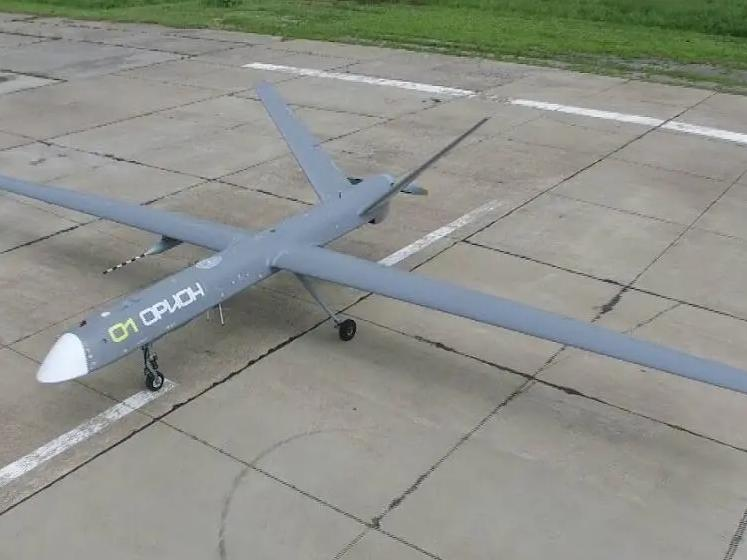
\includegraphics[width=6cm,height=5cm]{Fig/Orion.jpg}
		\caption{\label{Orion}猎户座固定翼无人机}
	\end{minipage}%
	\begin{minipage}[c]{0.5\textwidth}
		\centering
		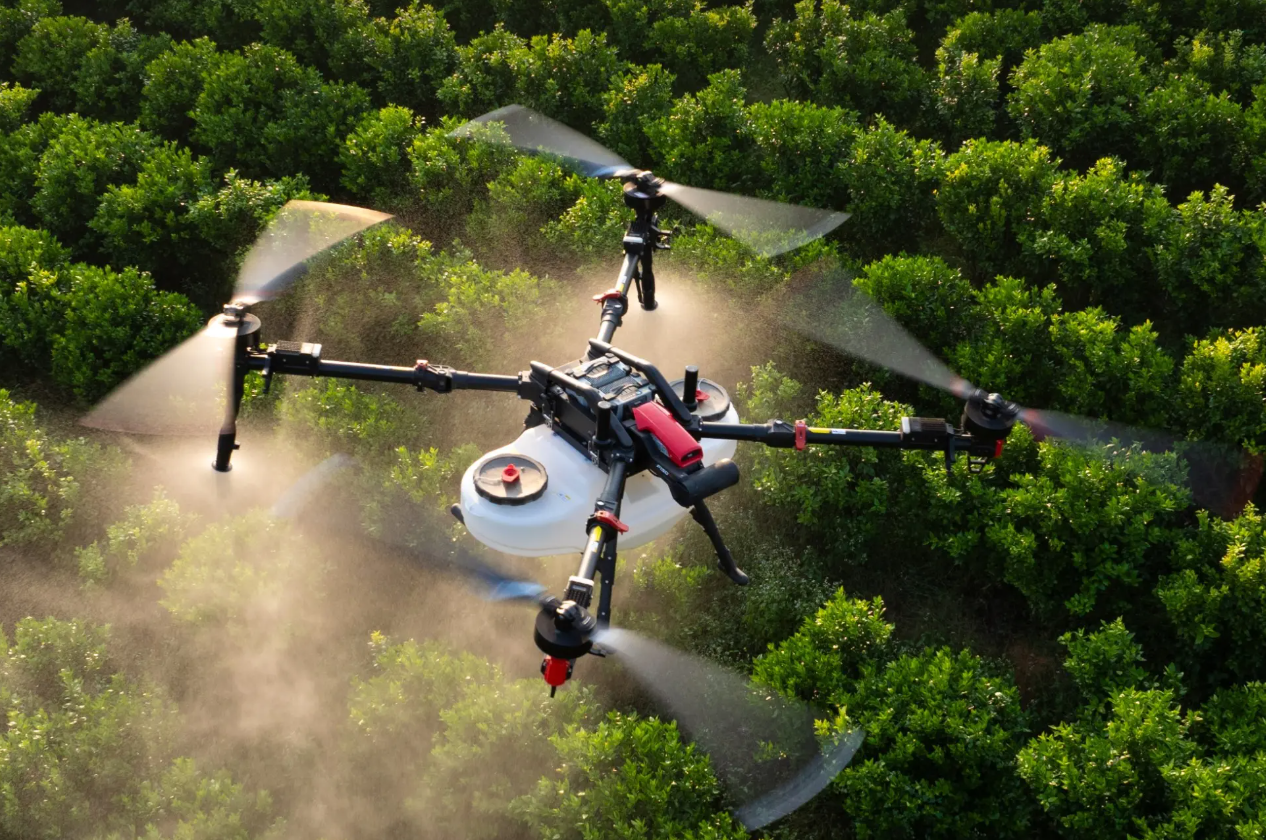
\includegraphics[width=6cm,height=5cm]{Fig/P150PRO.png}
		\caption{\label{P150PRO}极飞P150PRO农业无人机}
	\end{minipage}
\end{figure}

无人机发展百年,种类繁多,不同的任务需求驱动着创造不同类型的无人机。因此按照无人机的任务能力,可将其分为水平起飞着陆(Horizontal Take-off Landing,HTOL)、垂直起飞着陆(Vertical Take-off Landing,VTOL)、混合模型(倾转翼、倾转旋翼和涵道风扇)、直升机和非常规类型\cite{hassanalianClassificationsApplicationsDesign2017}。其中,涵道风扇无人机(Ducted Fan UAV,DFUAV)是指其螺旋桨被封闭在涵道内部的无人机,这些螺旋桨也被称为“风扇”,同时下方安装有若干控制舵面进行控制。DFUAV既有旋翼无人机般的垂直起降能力,又可以像固定翼无人机那样高速巡航,而且这种特殊的配置结构具有空气动力效率高和操作安全性的优势\cite{johnsonModelingControlFlight2006b,zhangReviewDuctedFans2020b,qianImprovingPerformanceDucted2022}。但不如人意的是,与开放旋翼相比,涵道风扇的罩状旋翼在飞行器周围的流场中会表现出强烈的耦合效应\cite{iiiNondimensionalModelingDuctedFan2012},并且由于其特殊的气动布局,DFUAV在垂直起降和水平巡航这两种不同的飞行模式下气动特性也完全不同\cite{johnsonModelingControlFlight2006b},这都对DFUAV的控制器设计提出了挑战。此外,针对DFUAV的轨迹规划的研究相对匮乏,这种研究的不足在一定程度上限制了DFUAV在复杂环境中的高效运作,不利于DFUAV的进一步推广应用。

正因如此,设计出适用于DFUAV的控制策略以及合理的轨迹规划方法,对于DFUAV的进一步发展具有重要意义。

\section{国内外研究现状}

\subsection{涵道风扇无人机}

目前已知的关于涵道风扇无人机的起源最早可以追溯到二十世纪三十年代,由意大利的Stipa和德国的Kort率先在该领域开展研究\cite{iiiNondimensionalModelingDuctedFan2012}。在二十世纪五十年代,美国宇航局在研究Doak VZ-4和Bell X-22涵道风扇垂直起降飞行器时投入了大量精力后取得一些进展,然而他们也发现了一些意料之外的特性,如从悬停到前飞过渡时,会出现机头上仰的趋势\cite{cookSummaryLiftLift1993}。Pereira等人\cite{pereiraHoverWindtunnelTesting2008}已经对涵道风扇早期的研究进行了详尽的回顾。近年来,随着先进的控制方法的提出和涵道风扇理论的进一步完善,涵道风扇无人机这一领域不仅引起了众多科研机构的广泛关注,还催生出了一系列具有里程碑意义的创新产品。

在二十世纪八十年代末期,美国Sikorsky航空公司试飞了一种名为“Cypher”的小型无人机。该无人机涵道直径1.75m,重量为20kg,采用共轴双桨结构提供动力,环形护罩在提升了拉力效率的同时也提升了其安全性。1992年4月,在初代Cypher的基础上,Cypher II进行了首次飞行。相比初代Cypher,Cypher II涵道直径1.9m,重量为110kg,并且在环形护罩外扩展了固定翼结构,并且尾部还有一个推进式螺旋桨,有效提升了Cypher II的飞行速度以及续航时间\cite{murphy1996air},最高时速可达230km/h,航程超过185km。

\begin{figure}[htbp]
	\centering
	\begin{minipage}[c]{0.5\textwidth} % minipage将页面划分为0.5\textwidth
		\centering
		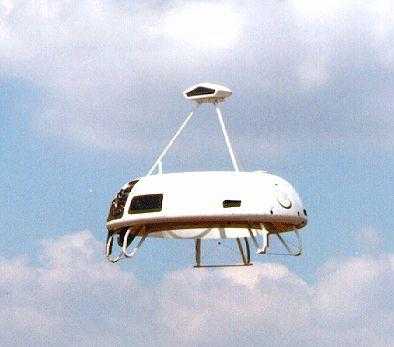
\includegraphics[width=6cm,height=5cm]{Fig/Cypher.jpg}
		\caption{\label{Cypher}Cypher}
	\end{minipage}%
	\begin{minipage}[c]{0.5\textwidth}
		\centering
		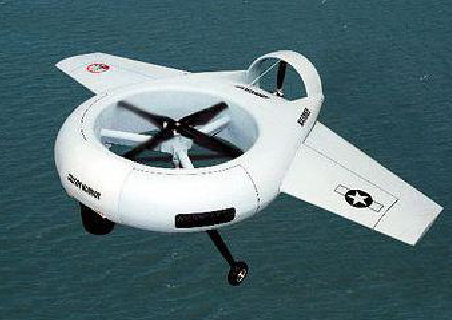
\includegraphics[width=6cm,height=5cm]{Fig/Cypher II.png}
		\caption{\label{Cypher II}Cypher II}
	\end{minipage}
\end{figure}

2003年,美国极光飞行科技公司根据国防高级研究计划局的“秘密无人机”计划开发了GoldenEye-100无人机,可垂直起降并且能携带11kg的有效载荷。次年7月,由GoldenEye-100衍生出的更小的GoldenEye-50无人机首飞。GoldenEye-50长70cm,翼展1.4m,最大飞行速度可达280km/h\cite{schaeferGoldenEyeClandestineUAV},并且在2005年4月进行了第一次自主水平飞行转换。GoldenEye-80是GoldenEye系列的第三个版本,长165cm,重达68kg,携带有高分辨率摄像机和激光测距仪等传感设备,设计意图用于满足美国陆军未来作战系统计划的要求。

2003年,Honeywell航空航天公司为美国陆军开发制造了RQ-16 T-Hawk微型无人机,并于2007年部署在了伊拉克战场上\cite{white2010upgrades}。该款无人机采用涵道风扇设计,涵道直径为35.5cm,总机重量为7.7kg,巡航速度可达74km/h,在战场上被广泛应用于可疑目标检查和跟随等任务。在2011年日本地震引发海啸进而导致核泄露后,4架T-Hawk被部署在福岛1号核电站,其机载的高分辨率摄像头拍摄了核电站受损部分的图像用于帮助日本核工程专家快速定位和解决问题。但是后来有两架T-Hawk在核反应堆上空坠毁,Honeywell公司并没有给出具体原因。

\begin{figure}[htbp]
	\centering
	\begin{minipage}[c]{0.5\textwidth} % minipage将页面划分为0.5\textwidth
		\centering
		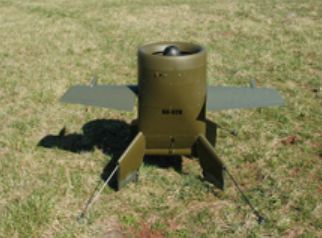
\includegraphics[width=6cm,height=5cm]{Fig/GoldenEye.png}
		\caption{\label{GoldenEye}GoldenEye}
	\end{minipage}%
	\begin{minipage}[c]{0.5\textwidth}
		\centering
		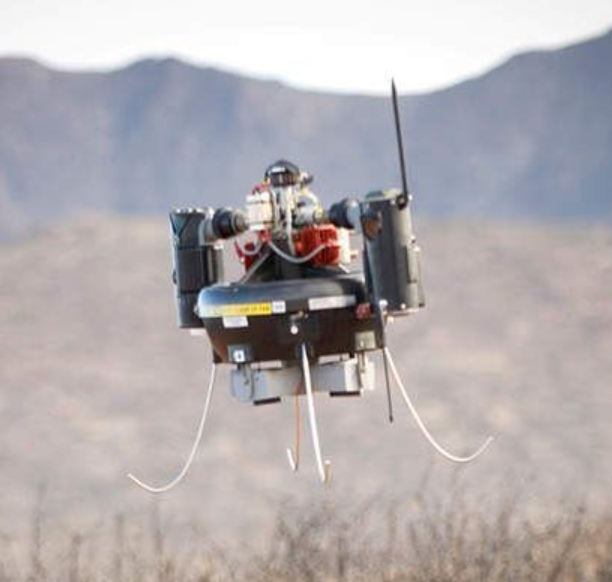
\includegraphics[width=6cm,height=5cm]{Fig/T-Hawk.png}
		\caption{\label{T-Hawk}T-Hawk}
	\end{minipage}
\end{figure}

2015年12月30日,由以色列Tactical Robotics公司研发的AirMule救护无人机首航。如图所示,AirMule的起飞旋翼设置在了机身内部,由涵道壁包裹,尾部还有两个推进涵道风扇用于控制姿态。这种构型专为直升机不方便起降的情形而设计,如山川、林地等地形复杂的区域。由于AirMule可负载80kg的载重能力和150km/h的最大速度\cite{yuTechnicalAnalysisVTOL2016},未来还将用于运输货物等任务。

\begin{figure}[htbp]
	\centering
	\begin{minipage}[c]{0.5\textwidth} % minipage将页面划分为0.5\textwidth
		\centering
		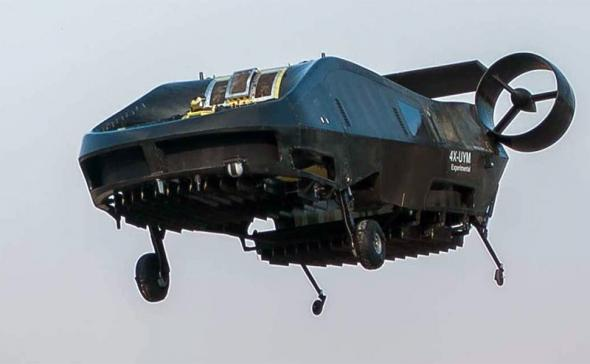
\includegraphics[width=7cm,height=5cm]{Fig/AirMule.jpg}
		\caption{\label{AirMule}AirMule}
	\end{minipage}%
	\begin{minipage}[c]{0.5\textwidth}
		\centering
		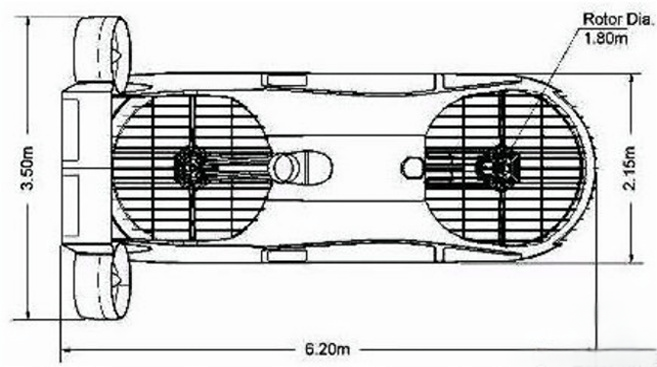
\includegraphics[width=7cm,height=5cm]{Fig/Airmule内部结构.png}
		\caption{\label{AirMule2}Airmule内部结构}
	\end{minipage}
\end{figure}

在2016年的HWTrek全球智能硬件创新与制造大会上,来自比利时无人机Fleye引发众人关注,如图所示。因其大小与篮球相当,许多媒体也把它称为“球形无人机”。Fleye也属于涵道风扇无人机的一种,摄像头安装在上部,下部为光流传感器,由于其安全小巧的特点,媒体预测其未来将会应用于室内摄影、娱乐等场合。除上述提到的采用涵道构型无人机外,还有由新加坡ST Aerospace研发的FanTail系列\cite{mateosanguinoDesignStabilizationCoanda2024}、Aesir公司的Odin\cite{crivoi2013survey}和美国联合宇航公司的iSTAR\cite{flemingImprovingControlSystem}等。

\begin{figure}[htbp]
	\centering
	\begin{minipage}[c]{0.33\textwidth} % minipage将页面划分为0.5\textwidth
		\centering
		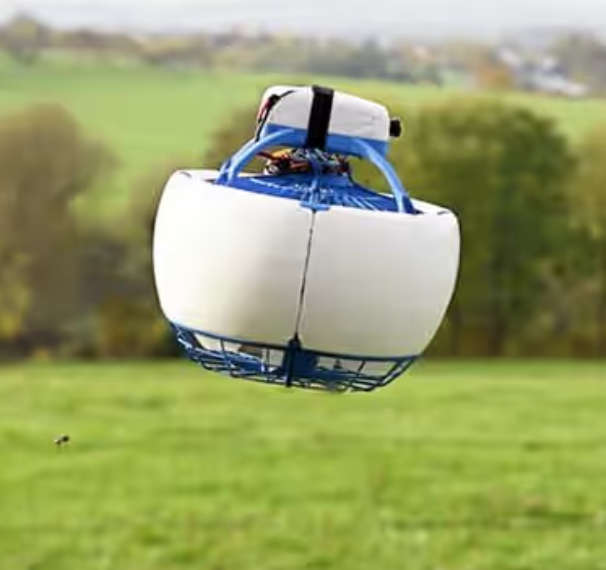
\includegraphics[width=5cm,height=5cm]{Fig/Fleye.png}
		\caption{\label{Fleye}Fleye}
	\end{minipage}%
	\begin{minipage}[c]{0.33\textwidth}
		\centering
		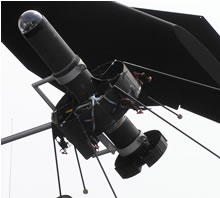
\includegraphics[width=5cm,height=5cm]{Fig/FanTail.png}
		\caption{\label{FanTail}FanTail}
	\end{minipage}
    \begin{minipage}[c]{0.33\textwidth}
		\centering
		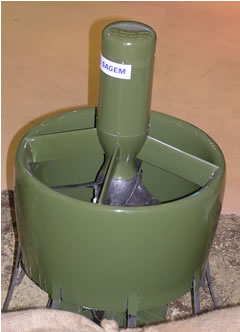
\includegraphics[width=4cm,height=5cm]{Fig/odin.jpg}
		\caption{\label{odin}Odin}
	\end{minipage}
\end{figure}

相较于国外的研究成果,我国涵道无人机研究起步相对较晚,大多处于实验探索阶段。2008年,哈尔滨盛世特种飞行器有限公司与中国航天科工集团第四研究院和哈尔滨工业大学航天学院合作共同研发制造出国内首例单桨环道“飞碟”,直径1.2m,续航40分钟,最大速度可达80km/h,并获得国家发明专利。由南昌航空大学设计的“都市精灵”涵道无人机获得2011年“中航工业杯—国际无人飞行器创新大奖赛”创意奖,其涵道直径1.2m,续航时间1h,最大飞行速度为50km/h。深圳千叶智能科技公司以研发涵道式无人机设计平台为主,目前已推出CDF-270、CDF-390和EDF-254等型号的无人机,可用于航拍、巡航和侦察等领域。

\begin{figure}[htbp]
	\centering
	\begin{minipage}[c]{0.33\textwidth} % minipage将页面划分为0.5\textwidth
		\centering
		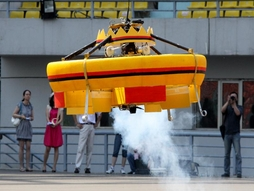
\includegraphics[width=5cm,height=5cm]{Fig/飞碟.jpg}
		\caption{\label{飞碟}飞碟}
	\end{minipage}%
	\begin{minipage}[c]{0.33\textwidth}
		\centering
		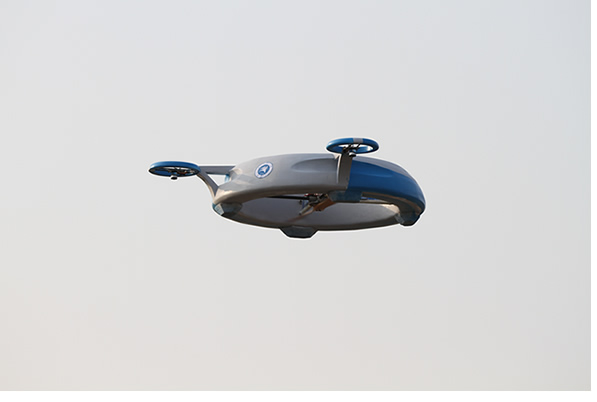
\includegraphics[width=5cm,height=5cm]{Fig/都市精灵.jpg}
		\caption{\label{都市精灵}都市精灵}
	\end{minipage}
    \begin{minipage}[c]{0.33\textwidth}
		\centering
		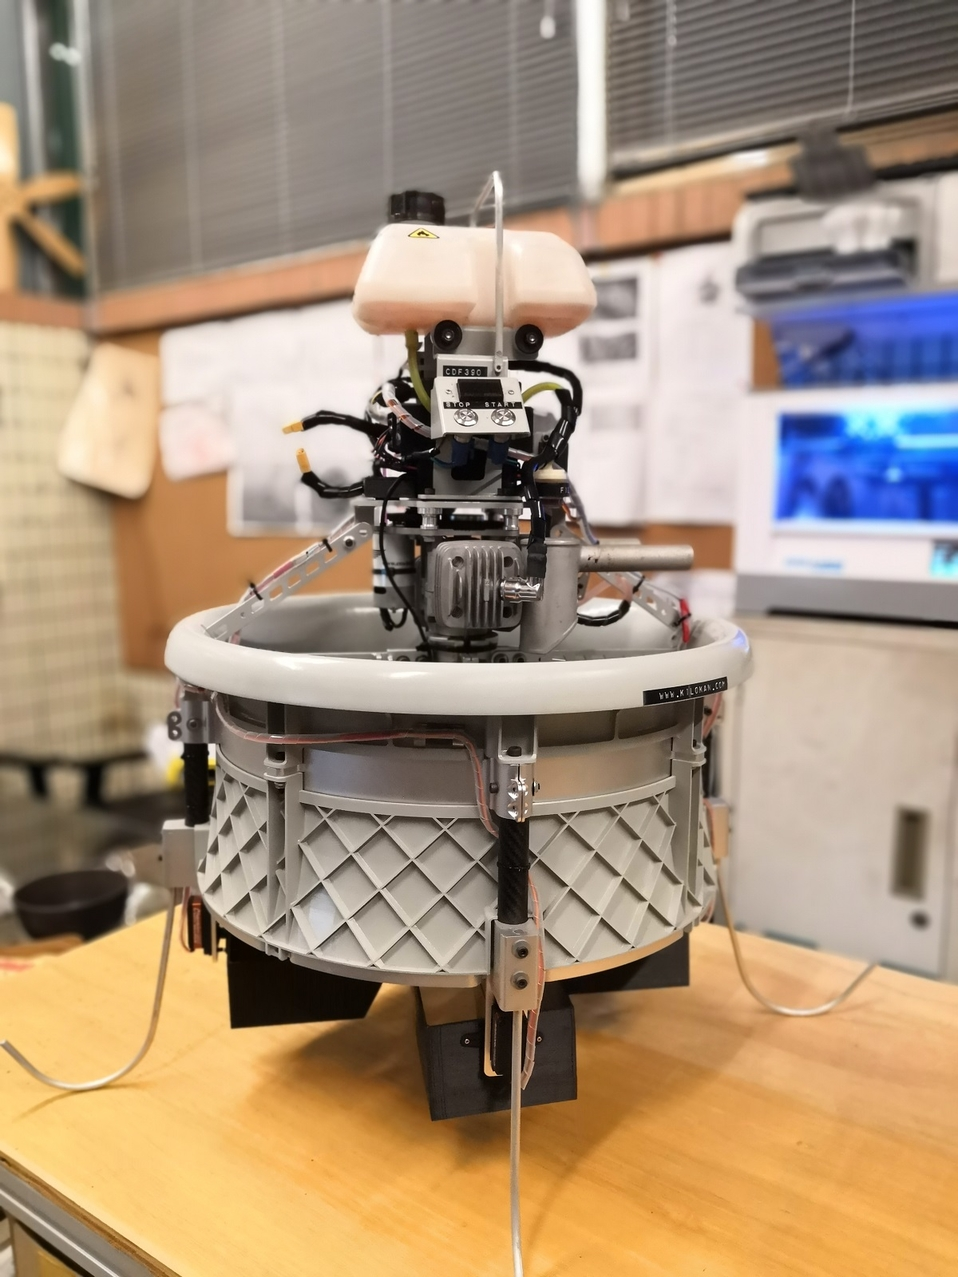
\includegraphics[width=4cm,height=5cm]{Fig/CDF-390.jpg}
		\caption{\label{CDF-390}CDF-390}
	\end{minipage}
\end{figure}

此外,清华大学\cite{chouStudyOverallDesign2021,luoNumericalAnalysisWind2024a}、北京理工大学\cite{manzoorCompoundLearningBasedModel2024}、南京航空航天大学\cite{caiNumericalPredictionUnsteady2022}和华南理工大学\cite{yinDuctedFanUAV2024,1022766347.nh}等高校也对涵道无人机展开了不同程度的研究,极大推动了我国在该领域的发展。

\subsection{飞行控制技术}

涵道风扇无人机的飞行控制技术是涵道风扇无人机研究的重要组成部分。飞行控制技术的研究主要包括控制器设计、轨迹规划和飞行仿真等方面。控制器设计是涵道风扇无人机飞行控制技服的核心,其目的是设计出一种能够使无人机在飞行过程中保持稳定的控制器。轨迹规划是指在给定的环境条件下,设计出一种使无人机能够按照预定的轨迹飞行的方法。飞行仿真是指利用计算机模拟无人机的飞行过程,以验证控制器设计和轨迹规划的有效性。

这里主要是想推荐一种“学术生态”,即利用各种工具展开科研工作,以达到事半功倍的效果。需要用到以下软件:
\begin{enumerate}[topsep = 0 pt, itemsep= 0 pt, parsep=0pt, partopsep=0pt, leftmargin=44pt, itemindent=0pt, labelsep=6pt, label=(\arabic*)]
	\item 	参考文献管理软件zotero\cite{_m}。很多人使用过endnote,但其实zotero也非常强大,强烈推荐。可到b站观看Struggle with Me出品的视频教程\cite{_k}入门(或其他最新教程,刚开始不推荐使用插件,会增加学习难度)。zotero自带pdf阅读器,也可以设置为使用其他阅读器。在zotero可以打开文件所在位置,故不推荐更改zotero的文件系统(尤其不推荐使用zotfile插件,事实上各种五花八门的插件增加了复杂性,实际上没有带来太多便利性)。理论上只需要包含文献元数据信息的bib文件(可以手动一篇一篇文章地收集)即可使用此模板,因此模板不依赖于任何参考文献管理软件,endnote用户或不使用参考文献管理软件的用户可以忽略本文zotero部分的讲解。
	\item	可截图获取文献中公式的软件mathpix\cite{_h}。在阅读别人的论文时,很可能需要把文章中的公式抄下来放到自己的笔记中,方便以后组会报告甚至论文中使用,这时使用mathpix可直接截图获取\LaTeX{}源码,非常方便。该软件普通邮箱注册可每月50次免费,学校邮箱可100次,若信用卡注册可1000次(最新情况是只能500次了,还要收费20美元,世界变化太快了)。注:随着mathpix的使用成本越来越高,免费次数越来越少,2023起已经不再推荐。目前开源/免费的替代工具为:。\href{https://www.simpletex.cn/}{SimpleTex}和\href{https://p2t.breezedeus.com/}{Pix2Tex}。目前SimpleTex性能比较好,免费但不开源,不排除未来收费的可能
	\item	TeXlive202x、TeXstudio,相当于开发环境和IDE。本模板是基于TeX的发行版TeXlive202x和编辑器TeXstudio进行的,百度这两个关键字分别安装。关于TeXstudio的使用(快捷键等)可另行查找资料。模板还支持更多ide,更多编译方式见GitHub首页readme.md。若在其他窗口打开了编译生成的pdf文件,记得关掉再编译,否则报错。TeXstudio的设置见第二章。
\end{enumerate}

本文的章节安排如下:

第一章,绪论。

第二章,模板简介。主要介绍各文件的内容。

第三章,常用环境。介绍论文写作中常用的环境,包括:图、表、公式、定理。基本涵盖了常用的命令。

%第三章,参考文献设置。本模板对旧版的改动主要是参考文献部分,本章将简单参考文献设置以及
%编译选项的设置等等。


